

\tikzset{every picture/.style={line width=0.75pt}} %set default line width to 0.75pt        

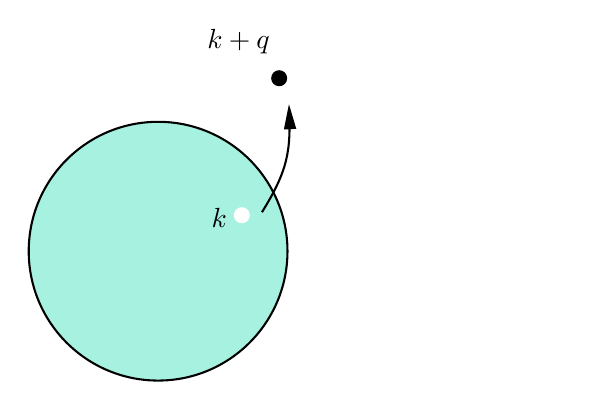
\begin{tikzpicture}[x=0.75pt,y=0.75pt,yscale=-1,xscale=1]
%uncomment if require: \path (0,300); %set diagram left start at 0, and has height of 300

%Shape: Circle [id:dp4394846235811054] 
\draw  [fill={rgb, 255:red, 80; green, 227; blue, 194 }  ,fill opacity=0.51 ] (186.33,148.33) .. controls (186.33,113.91) and (214.24,86) .. (248.67,86) .. controls (283.09,86) and (311,113.91) .. (311,148.33) .. controls (311,182.76) and (283.09,210.67) .. (248.67,210.67) .. controls (214.24,210.67) and (186.33,182.76) .. (186.33,148.33) -- cycle ;
%Straight Lines [id:da6443954751163439] 
\draw    (448,177) ;
%Straight Lines [id:da2953496654024814] 
\draw    (307,65) ;
\draw [shift={(307,65)}, rotate = 0] [color={rgb, 255:red, 0; green, 0; blue, 0 }  ][fill={rgb, 255:red, 0; green, 0; blue, 0 }  ][line width=0.75]      (0, 0) circle [x radius= 3.35, y radius= 3.35]   ;
%Straight Lines [id:da49388467901457345] 
\draw [color={rgb, 255:red, 255; green, 255; blue, 255 }  ,draw opacity=1 ][fill={rgb, 255:red, 255; green, 255; blue, 255 }  ,fill opacity=1 ]   (289,131) ;
\draw [shift={(289,131)}, rotate = 0] [color={rgb, 255:red, 255; green, 255; blue, 255 }  ,draw opacity=1 ][fill={rgb, 255:red, 255; green, 255; blue, 255 }  ,fill opacity=1 ][line width=0.75]      (0, 0) circle [x radius= 3.35, y radius= 3.35]   ;
%Curve Lines [id:da7891006108897265] 
\draw    (298.71,129.55) .. controls (311.32,109.18) and (312.64,100.1) .. (311.79,79.5) ;
\draw [shift={(311.71,77.55)}, rotate = 447.4] [fill={rgb, 255:red, 0; green, 0; blue, 0 }  ][line width=0.08]  [draw opacity=0] (12,-3) -- (0,0) -- (12,3) -- cycle    ;

% Text Node
\draw (304,55) node [anchor=south east] [inner sep=0.75pt]    {$\boldsymbol{k} +\boldsymbol{q}$};
% Text Node
\draw (273,126) node [anchor=north west][inner sep=0.75pt]    {$\boldsymbol{k}$};


\end{tikzpicture}
